\documentclass[12pt]{article}
\usepackage[utf8]{inputenc}
\usepackage{graphicx}
\usepackage{wrapfig}
\usepackage{setspace}
\usepackage{array}
\graphicspath{ {images/} }
\usepackage{lipsum}
\usepackage{ragged2e}
\usepackage{pythonhighlight}
\newcolumntype{C}[1]{>{\centering\let\newline\\\arraybackslash\hspace{0pt}}m{#1}}
\newcolumntype{L}[1]{>{\raggedright\let\newline\\\arraybackslash\hspace{0pt}}m{#1}}
%%%%%%%%%%%%%%%%%%%%%%%%%%%%%%%%%%%%%%%%%%%%%%%%%%%%%%%%%%%%%%%%%%%%%%%%%%%%%%%%%%%%%%%%%%%%%%%%%%%%%%%%%
%%%%%%%%%%%%%%%% HEADER PART %%%%%%%%%%%%%%%%%%%%%%%%%%%%%%%%%%%%%%%%%%%%%%%%%%%%%%%%%%%%%%%%%%%%%%%%%%%%
\usepackage[a4paper,right=1.0in,top=1in,bottom=1in,left = 1.0in,width=150mm,bindingoffset=6mm]{geometry}
\begin{document}
	% !TEX root = ../thesis-example.tex
%
% ------------------------------------  --> cover title page
\begin{titlepage}
%	\pdfbookmark[0]{Cover}{Cover}
	\begin{center}
	\hfill
	
   
	\rule[5pt]{\textwidth}{1.0pt} \par
{\Huge \textbf{DevOps Tools Training at Dell EMC} \par}
\rule[5pt]{\textwidth}{1.0pt} \par

	\vspace*{1cm}
	{\large \fontfamily{ppl}\centering\textit{An Industrial Internship Training Report}\par \vspace*{1cm}
	\textit{submited to}\par
		{\Large JSS Science \& Technology University} \par  
		{
\includegraphics[width=0.4\textwidth]{logo.jpg}} \par
		{\textit{for the fulfillment of the requirements for the degree of \\ Master of Technology}\par in \par\textit{Data Science} \par	\vspace*{1cm}
			\vspace*{2cm}
			\textit{submited by} \hfill \textit{Mentor}\par
			\vspace*{0.5cm}
			\textit{Kishore G R} \hfill \textit{Gourishankar Mohapatra,}\par
			\textit{USN - 01JST19PDS005} \hfill \textit{Manager, Software Engineer,}\par
			\hfill \textit{Dell EMC, Bagmane Tech Park, Bengaluru.}\par
            \hfill \textit{Gourishankar\_Mohapatra@Dell.com}
	    \vfill
	    \large\fontfamily{ppl} {Department of Information Science \& Engineering}\par
		\small \fontfamily{ppl}{JSS Science \& Technology University (SJCE), Mysuru}} 

	\vfill
}
%	\textit{\large\Submitted by} \\
%	Version: \thesisVersion
	\end{center}
\end{titlepage}


% ------------------------------------  --> main title page
%\begin{titlepage}
%	\pdfbookmark[0]{Cover}{Cover}
%	\flushright
%	\hfill
%	\vfill
%	{\LARGE\thesisTitle \par}
%	\rule[5pt]{\textwidth}{.4pt} \par
%	{\Large\thesisName}
%	\vfill
%	\flushleft
%%	\textit{\large\thesisDate} \\
%	 Copyright \copyright \the\year \par
%	Permission is granted to copy, distribute and\slash or modify 
%	this document under the terms of the GNU 
%%	Version: \thesisVersion
%\end{titlepage}


% ------------------------------------  --> lower title back for single page layout
%\hfill
%\vfill
%{
%	\small
%	\textbf{\thesisName} \\
%%	\textit{\thesisTitle} \\
%%	Department of Information Science \& Engineering\thesisSubject, \thesisDate \\
%%	Reviewers: \thesisFirstReviewer \\
%%	Supervisors: \thesisFirstSupervisor \\[1.5em]
%%	{Department of Information Science \& Engineering} \\
%%	\textit{\thesisUniversityGroup} \\
%	\thesisUniversityDepartment \\
%	\thesisUniversityInstitute \\
%	\thesisUniversityStreetAddress \\
%	\thesisUniversityPostalCode\ \thesisUniversityCity
%}

	\begin{center}
\emph{\LARGE\textbf {Certificate}}\\[2.5cm]
\end{center}


\doublespacing
This is to certify that Mr. \textit{Kishore G R} from the M.Tech in Data Science Department of JSS Science \& Technology University, Mysuru has completed the Industrial Training under my supervision. He was trained in the field of \textit{DevOps Build Tools} from July 20, 2020 to July 16, 2021 for the academic year 2020-2021. His works is found satisfactory. 

\vspace*{4cm}

%hfill (space for signature)\par
\hfill \textit{Gourishankar Mohapatra,}\par
\hfill \textit{Dell EMC, Bagmane Tech Park, Bengaluru.}\par
\hfill \textit{Gourishankar\_Mohapatra@Dell.com}

	\newpage
	\tableofcontents
	\newpage
	\listoffigures
	\newpage
	\section{Introduction}
	
In recent years, DevOps has become a popular choice for the software development process; it offers a set of practices which result in better and faster software development cycle with high software quality by enabling the Agile development. Nowadays most of the organisations follow DevOps Practices for the software development.

Before DevOps, the commonly used software development model was WATERFALL model. This model is best suited when all the requirements are available at the planning stage of the development cycle i.e., all the requirements provided must be finalised, no later changes or additions are entertained in this model and no work is performed in parallel, thus making the software life cycle very long.

\begin{figure}[htbp]
\begin{center}
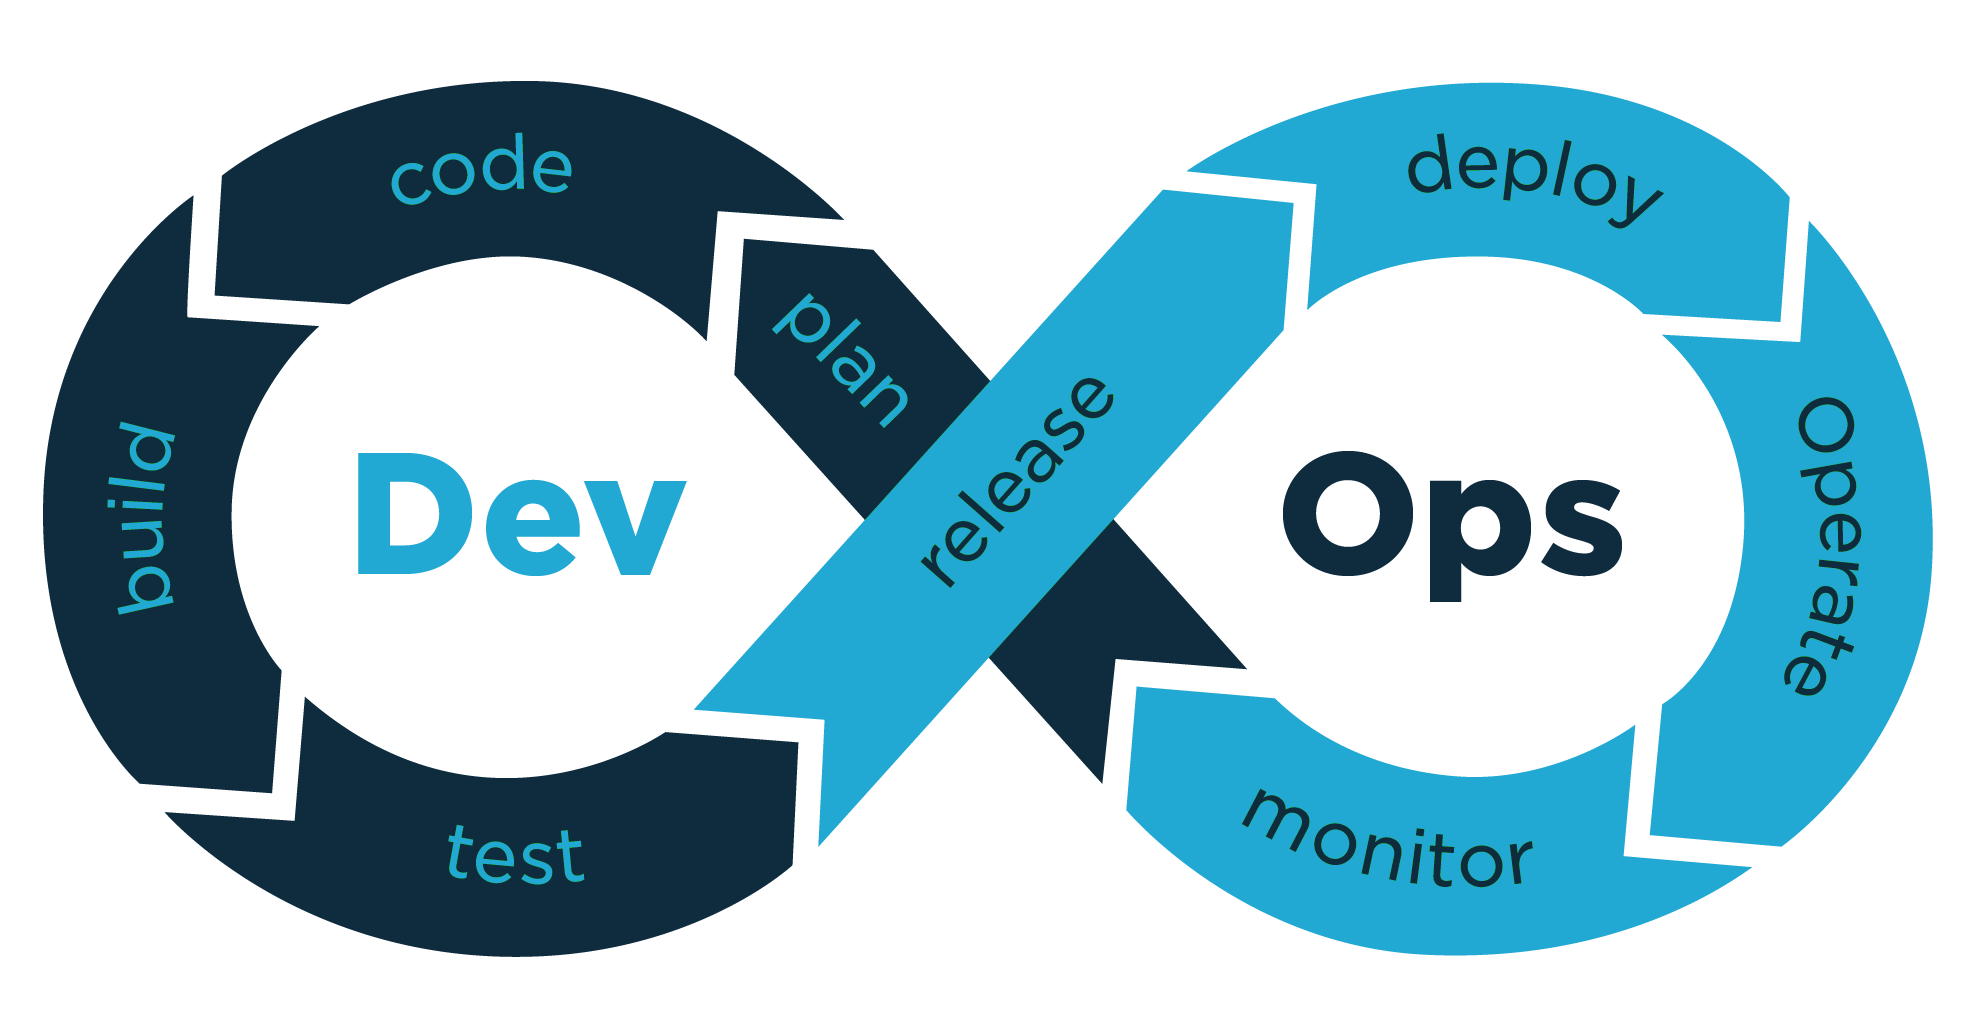
\includegraphics[width=0.9\textwidth]{devops.png}
\end{center}
\caption{DevOps Flow}
\end{figure}
\begin{center}
\tiny [Image Source: DevOps in a Scaling Environment by Medium]
\end{center}


DevOps offers a continuous integrated build mechanism, where it allows \textbf{Continuous Business Planning} which enables placing of new feature requirements at any point of time which will be handled by \textbf{Collaborative Development process} where the development of each feature will be handled by different teams independently with the help of Version Control tool such as Git. Each feature is \textbf{Continuously Tested} and Verification and validation tests can be done by Jenkins server using different test tools. Once the product is production ready, the continuous integration mechanism of DevOps helps in \textbf{Continuous Release and Deployment} of the application, then the performance of the application and the state of the servers are kept track by \textbf{Continuous monitoring systems}. Finally, the \textbf{Collaborative Customer Feedback and Optimization} helps in getting feedbacks from a specific customer base on the released feature which is considered to be very important in DevOps cycle because it helps the developer to provide changes in features accordingly and deployment engineer to understand the server configuration required for smooth conduct of the service. 

In my training program, I have been introduced to some of the devOps tools, where I get to work with tools such as Docker, Kubernetes, Jenkins, JFrog Artifactory and Git.
	
	\subsection{About the organization}
	
Dell EMC, formerly known as EMC Corporation is an American multinational corporation head quartered in Hopkinton, Massachusetts and Texas. EMC was acquired by Dell in 2016, and it is a Product based company that mainly focuses on Data Storage, information security, virtualization, cloud computing and other products and services that enables organizations to store, manage protect and analyze data. 

EMC was noted by Forbes for its "focus on developing and selling data storage and data management hardware and software and convincing its customers to buy its products independent of their other IT buying decisions".

Dell Technology is at the forefront of driving digital future and is committed to innovate and develop technology that transforms business, thus helping organisations to progress in much more effective way. The brands parented by Dell Technologies are Dell, Dell EMC, Secureworks, virtustream and VMware, with the combined power of these industry leaders Dell technologies aims to harness the digital transformation in a global scale.

Dell technologies also believe in advancing sustainability, where it ensures everyone’s responsibility to protect and enrich our planet together with customers, suppliers and communities. Besides, by 2030 for every product a customer buys, Dell aims to reuse or recycle an equivalent product, and 100\% of packaging will be made from recycled or renewable materials.	
	
	\subsection{About the work carried out}
	
As mentioned in the previous section, Dell EMC mainly focuses on Infrastructure solutions where it deals with storage, servers and networking, cloud solutions and data protection related products and services. Here I have been assigned to DevOps organisation specifically the team that handles devOps build tools.

Initially, as a part of training I was allowed to get myself familiar with some of the tools with which I will be working on during my internship, such as Docker, Kubernetes, AQL and Jenkins (which are explained in detail in section 1.3). I learned, and understood the use and working of these tools from various sources and implemented both demo and scenario based use cases using these tools. The implementation has helped me in getting more insight about these tools, their behaviour for different configurations and how each tool can be used effectively for better deployment of a software application.

My major work till now involves Docker and Kubernetes; along with these applications some of the tasks required python, groovy, Go and NodeJS programing knowledge where I improved my knowledge in few languages and learnt few languages from scratch and I was introduced to some of the tools such as jira and Jfrog platforms.	
	
	\subsection{DevOps tools and Languages Trained}

\begin{tabular}{C{3.8cm}  L{10.7cm}}
        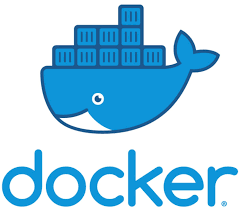
\includegraphics[width=3.7cm]{docker.png} & {\Large{\textbf{Docker}}} \newline 
        Docker is a containerization tool that helps in isolating a process from rest of the processes that are running in a system, where it bundles application code, support binaries and configuration together.
\end{tabular}	
To give a better distinction between Virtual Machines and Containers let’s have a look at how isolation take place between both.	



\begin{figure}[htbp]
\begin{center}
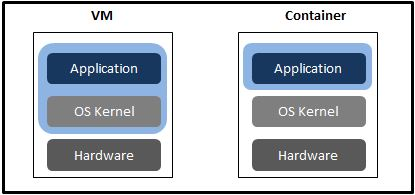
\includegraphics[width=0.7\textwidth]{vm.jpg}
\end{center}
\caption{Virtual machine V/s Container}
\end{figure}

In VMs the Application and the OS kernel layers are abstracted, that is every new VM contains its own kernel but they all share same host hardware which is resource expensive. But in case of containers, it is the abstraction of application layer which is light weight in nature.\\


\begin{tabular}{C{3.8cm}  L{11cm}}
        
\includegraphics[width=3.8cm]{k8s.png} & {\Large{\textbf{Kubernetes}}} \newline 
        Kubernetes is a container orchestration tool, that is; it helps in automating deployment, scaling and management of containerized application.This is done by grouping the
\end{tabular}
   containers into logical units for easy discovery and management.

To give a basic understanding on how Kubernetes works, let’s consider the scenario shown in Figure 3.

\begin{figure}[htbp]
\begin{center}
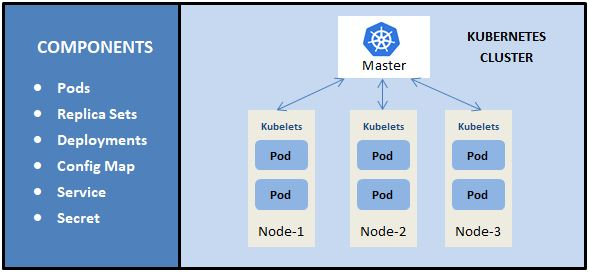
\includegraphics[width=1\textwidth]{kube.jpg}
\end{center}
\caption{Kubernetes Componenets and cluster visualization}
\end{figure}

Here, every Kubernetes deployment will have the cluster that contains both master and worker nodes,There can be any number of masters depending on the requirement. Pods are the smallest objects that represent a single instance of a running process in a cluster. Pods can contain one or more containers which are considered as single entity that shares resources allocated to a pod.

Each node in a cluster contains a Kubernetes agent called as kubelets in it, which keeps track of all the pods and their status, which are updated to the master frequently. Pods are not run in master nodes; they are only to be deployed in worker nodes.

Components that are listed are the ones for which the developer needs to write a manifest file, where:
\begin{enumerate}
\item Pods: it is a specification of a pod, such as container image to be used, port and other details.
\item Replica Sets: it is a specification file that contains pod details along with number of replications of a pod.
\item Deployment: it is similar to Replica sets but, when a replica set is deleted then the deployment creates replica sets with exact same specification.
\item Service: it is a specification file that helps in port mapping and communication between the pods.
\item Secret/ConfigMap: these are specification files that help in storing credentials and environment variables that are commonly used by a deployment pods in a single location.

\end{enumerate}


\begin{tabular}{C{3.8cm}  L{10.2cm}}
        
\includegraphics[width=3.6cm]{jfrog.jpg} & {\Large{\textbf{Jfrog}}} \newline 
\justify 
Jfrog is an artifacts management tool; it helps in maintaining the build artifact and dependencies from development to production in a universal artifact repository of a company thus providing support to devOps
\end{tabular}
platform and pipeline security. 

In order to handle the artifacts user can use either User Interface (UI) or Jfrog CLI. In case of CLI, Artifactory Query Language (AQL) is used to perform operations on the artifacts.

When the AQL query is given in the form of JSON spec file, the spec file contains the following properties.

\begin{python}
{
    "files": [
        {
            "pattern" or "aql": "[Mandatory]",
            "props": "[Optional]",
            "excludeProps": "[Optional]",
            "recursive": "[Optional, Default: 'true']",
            "exclusions": ["[Optional, Applicable only when 'pattern' is specified]"],
            "archiveEntries": "[Optional]",
            "build": "[Optional]",
            "bundle": "[Optional]",
            "sortBy" : ["[Optional]"],
            "sortOrder": "[Optional, Default: 'asc']",
            "limit": [Optional],
            "offset": [Optional]
        }
    ]
}

\end{python}


\begin{tabular}{C{3.8cm}  L{10.2cm}}
        
\includegraphics[width=3.8cm]{jenkins.jpg} & {\Large{\textbf{Jenkins}}} \newline 
\justify 
Jenkins is an open source automation server based system, which helps in accelerating the different parts of software development process such as building, testing, and deploying thus facilitating continuous integration 
\end{tabular}
and continuous delivery.

Every task in Jenkins is considered as job and the process is called as build, the jobs can be initiated in two ways either through UI or by using Jenkins configuration file. The Jenkins build instructions are written using Groovy script.
	\newpage
	\section{Assignments Taken Up}
	
Since the training mostly focuses on DevOps Tools, I have been assigned with tasks that mostly use the tools mentioned in section 1.3 of this report. One task is to deploy a NodeJs application where one gets to know about Docker, K8s and NodeJs and the other one helps in knowing how to use Jenkins, AQL and Jfrog Platform for development purpose	
	
	\subsection{Deployment of NodeJS application using Kubernetes and to perform Liveness Probe on it}
	
	
	\subsubsection{Introduction}
	
This task helps in implementing a mechanism offered by the Kubernetes to handle failed pods and avoid any events which reduces the performance of the deployment of the application, thus by maintaining the pods in a healthy state.	
	
	\subsubsection{Design work-flow}

\begin{figure}[htbp]
\begin{center}
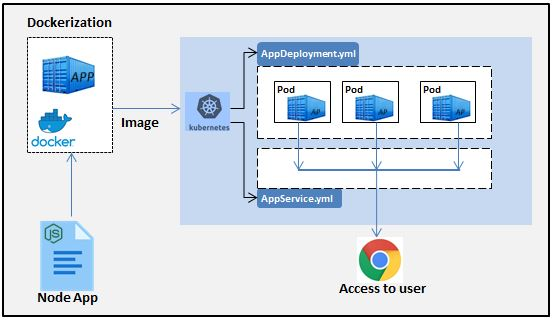
\includegraphics[width=1\textwidth]{flow1.jpg}
\end{center}
\caption{Deployement Flow}
\end{figure}

The flow of the project starts from NodeJS application, \\
a. Firstly the NodeJs app is dockerized, i.e., the docker image of the application is built. \\
b. Then, the manifest files for the components Deployment and Service are prepared (AppDeployment.yml and AppService.yml from image), where the previously built docker image of the NodeJs application is used for the container of the pod. \\
c. Finally, the Deployment and Service are created thus by making the application active and accessible to the external world.\\
 \textit{[In this case, the replica count is 3 i.e., three pods will be deployed for the service]}

	\subsubsection{Liveness probe}
	
	The liveness probe is one of many probes offered by Kubernetes that deals with the health of the pod. In liveness Probe the pods that stops due to some glitches and fails to respond to the request will be restarted, thus maintaining all the pods deployed in Ready state.	
	
	\subsection{Jenkins freestyle project to download artifacts}
	

	
	\subsubsection{Introduction}
	
This task is straight forward, where the Spec file of the AQL query is fed to Jenkins job and all the artifacts that match with the conditions in query are downloaded.		
	
	\subsubsection{Design work-flow}

\begin{figure}[htbp]
\begin{center}
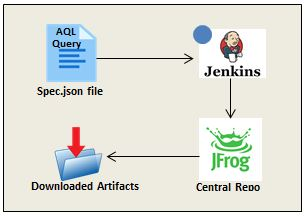
\includegraphics[width=0.8\textwidth]{jj.jpg}
\end{center}
\caption{Build Flow}
\end{figure}	
	
The steps are as follows:\\
a.	Firstly, The Spec.json file needs to be created with an appropriate AQL query.\\
b.	Then, the Spec file is fed as input to the Jenkins freestyle project; here the Jenkins Artifactory plugins is a Pre-requisite, without which on cannot connect to Artifactory management tool.\\
c.	Finally, when the job runs successfully, the artifacts that match the conditions specified in AQL are downloaded to the local system from the central repository of the organization. 
	
	
	\subsection{Other tasks}
Some of the other tasks that I have been assigned are as follows:	
\begin{itemize}


  \item  Perform readiness probe on Kubernetes pod deployment. 
  \item  Upload, download and search artifacts with and without properties using AQL query.
  \item  Create a Python script that takes a text file (containing the artifacts path) as input and downloads all the mentioned artifacts.
  \item Along with tasks, we get to learn about few other skills such as, how one should prepare a PPT presentation and how to deliver the content.

\end{itemize}	
	
	
	\newpage
	\section{Conclusion}
	\subsection{Briefly summarize the work done}
	
During my internship I was assigned with projects which were mostly related to devOps and these projects required fundamental knowledge about few of the industry standard tools which are already discussed in the previous sections of this report.

Though the tools mentioned were new to me, constant support from my mentor and team members made it easier for me to understand the use of tools and working with them was never been easier for me. The tasks on which I worked have thought me many techniques and efficient ways to handle a software project. Some of the assignments have made me learn new things and some improved my knowledge on previously known topics.	
	
	
	\subsection{Impact of industrial training}
	
Firstly, the industrial training has helped me in realizing the gap between the technical knowledge possessed by a student and a professional software engineer. The internship has helped me in understanding,
\begin{itemize}
  \item How an organization works, and how the roles are divided.
 \item How team members work together to meet the goal.
 \item How knowledge sharing takes place in organisations.
 \item How plans and strategies are discussed during meetings.
 \item How one should follow companies code of conduct to maintain a productive ambience in the organisation.
\end{itemize} 

Along with above mentioned perks, some of the periodically conducted webinars helped in improving my soft skills and some sessions helped in improving technical skills.
The entire industrial training can be concluded as a fruitful journey where I both gained from the company and contributed to the company.	
	
	\addcontentsline{toc}{section}{References}
	
	\begin{thebibliography}{9}
		\bibitem{Docker} 
		Docker tutorials 
		\\\texttt{https://www.docker.com/101-tutorial}
		
		\bibitem{Kubernetes} 
		Kubernetes tutorials 
		\\\texttt{https://kubernetes.io/docs/home/}
		
		\bibitem{AQL} 
		AQL Documentaion 
		\\\texttt{https://www.jfrog.com/confluence/display/JFROG/Artifactory+Query+Language}
		
		\bibitem{jenkins} 
		Jenkins tutorials 
		\\\texttt{https://www.jenkins.io/doc/tutorials/}
		
		\bibitem{Dell} 
		Dell Technologies information 
		\\\texttt{https://www.delltechnologies.com/en-in/index.htm}
		
		
	\end{thebibliography}
	
	
\end{document}
